\documentclass[12pt,a4paper]{article}

% ===== PAKETE =====
\usepackage[ngerman]{babel}          % Deutsche Sprache
\usepackage[utf8]{inputenc}          % UTF-8 Kodierung
\usepackage[T1]{fontenc}             % Schriftkodierung
\usepackage{lmodern}                 % Schönere Schrift
\usepackage[left=2.5cm,right=2.5cm,top=2.5cm,bottom=2.5cm]{geometry}

% Layout & Formatierung
\usepackage{setspace}                % Zeilenabstand


\usepackage{parskip}                 % Absatzformatierung
\usepackage{fancyhdr}                % Kopf- und Fußzeilen

% Bilder & Grafiken
\usepackage{graphicx}                % Bilder einbinden
\usepackage{float}                   % Bessere Positionierung
\usepackage{caption}                 % Bildunterschriften

% Tabellen
\usepackage{tabularx}                % Flexible Tabellen
\usepackage{booktabs}                % Schönere Tabellen

% PDF einbinden
\usepackage{pdfpages}                % Für Deckblatt

% Mathematik (falls benötigt)
\usepackage{amsmath}
\usepackage{amssymb}
\usepackage{siunitx}

% Links & Verweise
\usepackage{hyperref}                % Klickbare Links
\hypersetup{
    colorlinks=true,
    linkcolor=black,
    citecolor=black,
    urlcolor=blue,
    pdftitle={Titel deiner Arbeit},
    pdfauthor={Dein Name}
}

% Literaturverzeichnis
\usepackage[backend=biber,style=numeric,sorting=nty]{biblatex}
\addbibresource{literatur.bib}

% ===== EINSTELLUNGEN =====
\onehalfspacing                      % 1,5-facher Zeilenabstand
\setlength{\parindent}{0pt}          % Keine Einrückung
\pagenumbering{arabic}

% Kopf- und Fußzeilen
\pagestyle{fancy}
\fancyhf{}
\fancyhead[L]{\leftmark}
\fancyhead[R]{\thepage}
\renewcommand{\headrulewidth}{0.4pt}

% ===== DOKUMENT =====
\begin{document}

% Vorgegebenes Deckblatt einbinden
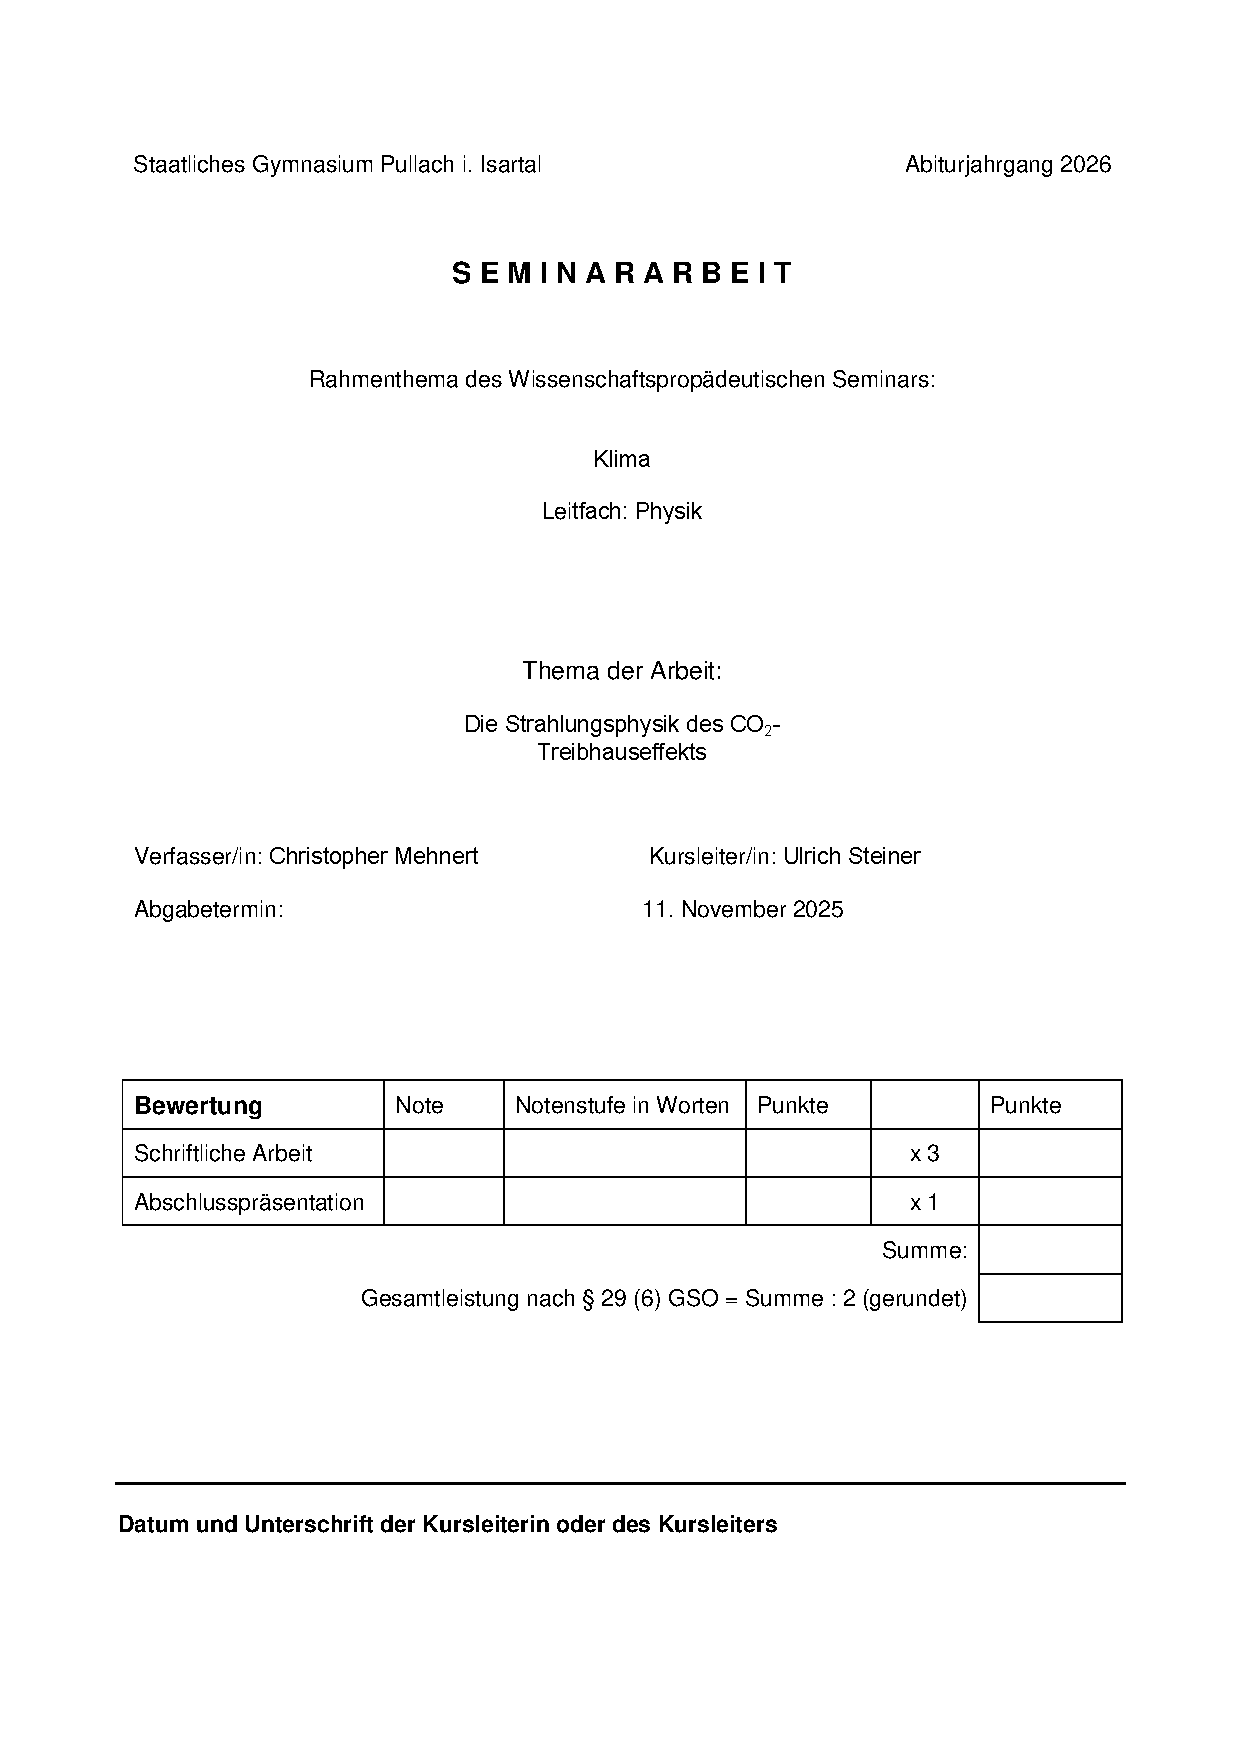
\includepdf[pages={1,2,3}]{assets/deckblatt.pdf}


% Inhaltsverzeichnis
\setcounter{page}{2}
\tableofcontents
\newpage

% Optional: Abbildungsverzeichnis
% \listoffigures
% \newpage

% Optional: Tabellenverzeichnis
% \listoftables
% \newpage

% ===== HAUPTTEIL =====

\section{Einleitung}

\section{Physikalische Grundlagen der Wärmestrahlung}

\subsection{Strahlungsgesetze}

\subsubsection{Das Plancksche Strahlungsgesetz}
Die spektrale Energiedichteverteilung der Hohlraumstrahlung wird durch das Plancksche Strahlungsgesetz beschrieben.
Die spektrale spezifische Ausstrahlung $B_f(T)$ eines schwarzen Körpers als Funktion der Frequenz $f$ und der Temperatur $T$
lautet nach Plank (1900) \cite{plancknormalspektrum}\cite{plancknormalspektrumtheorie}:

\begin{equation}
  \label{Spektrale Strahldichte als Funktion der Wellenlänge}
    B_f(T) = \frac{2hf^3}{{c_0}^2} \cdot \frac{1}{e^{hf/kT}-1} \quad \text{\cite{lmuplanck}}
\end{equation}


Alternativ kann die spektrale Strahldichte als Funktion der Wellenlänge $\lambda$ formuliert werden:
\begin{equation}
  \label{Spektrale Strahldichte als Funktion der Wellenlänge}
    B_{\lambda}(T) = \frac{2h{c_0}^2}{\lambda^5}\cdot \frac{1}{e^{hc_0/\lambda kT}-1} \quad \text{\cite{lmuplanck}}
\end{equation}

Hierbei bezeichnet $h = \SI{6.626e-34}{\joule\second}$ das Plancksche Wirkungsquantum, $c = \SI{2.998e+8}{\meter\per\second}$
die Vakuumlichtgeschwindigkeit und $k = \SI{1.381}{\joule\per\kelvin}$ die Boltzmann-Konstante \cite{codata2018}

\subsubsection{Das Stefan-Boltzmann Gesetz}
Eine Ober


\subsection{Anwendung auf das System Sonne-Erde}

\section{Molekülphysik des CO\textsubscript{2}}

\subsection{Molekülstruktur und Schwingungsmoden}

\subsection{Quantenmechanische Grundlagen der Absorption}

\subsection{Das CO\textsubscript{2}-Absorptionsspektrum}

\section{Der Treibhauseffekt}

\subsection{Strahlungsbilanz der Erde ohne Atmosphäre}

% ===== LITERATURVERZEICHNIS =====
\newpage
\section{Anhang}

\subsection{Literaturverzeichnis}
\printbibliography[heading=none]

% ===== ANHANG (optional) =====
% \newpage
% \appendix
% \section{Zusätzliche Daten}
% ...

\end{document}